\chapter{Analyse der Aufgabenstellung}
\label{sec:analyse-der-aufgabenstellung}

Die Aufgabenstellung hat zum Ziel (siehe Anhang \ref{sec:aufgabenstellung}, ``\nameref{sec:aufgabenstellung}''), Architekturkonzepte anhand einer Beispielapplikation darzustellen und diese in das Modul Internettechnologien zu transferieren. Sie verzichtet dabei bewusst auf funktionale Anforderungen an die zu erstellende Applikation. Weiter werden auch keine spezifischen Technologien zur Umsetzung vorgegeben.

Diese sehr offene Ausgangssituation wird lediglich durch die folgenden Ansprüche eingegrenzt:

\begin{enumerate}
	\item Das Produkt soll unter Verwendung einer oder mehreren Internettechnologien konzipiert und umgesetzt werden.
	\item Der zu erstellende Quellcode soll \emph{State Of The Art} Architekturprinzipien (\cite{ROCA} \& \cite{TilkovSlides}) exemplarisch darstellen und der interessierten Fachperson als auch Studenten der Vorlesung \emph{Internettechnologien} als Anschauungsmaterial dienen können.
\end{enumerate}

Von diesen zwei Leitsätzen ausgehend kann angenommen werden, dass die Demonstration von Architekturprinzipien klar im Vordergrund stehen soll. Da diese Prinzipien aber auch einem lernenden Publikum (Punkt 2) so interessant wie möglich präsentiert werden sollen, ist eine attraktive Verpackung ebenfalls nicht zu vernachlässigen.

Dieses Kapitel beantwortet im weiteren Verlauf dementsprechend folgende Fragen genauer:

\begin{enumerate}
	\item Wie werden die vorgegebenen Architekturprinzipien am optimalsten auf eine Beispielapplikation abgebildet?
	\item Welche Schritte wurden im Bereich der Entwicklung der Applikationsidee (\nameref{sec:produktentwicklung-einleitung}) durchlaufen? Auf welche Aspekte wurde besonders eingegangen?
	\item Wie wurde die Technologie zur Umsetzung der generierten Produktidee ausgewählt und welche Kriterien waren dabei ausschlaggebend?
	\item Kann mit der Evaluierten Technologie ein verwendbarer Prototyp angefertigt und ein ``\gls{ProofOfConcept}'' erbracht werden?
\end{enumerate}

\newpage
\section{Architekturrichtlinien}
\label{sec:architekturrichtlinien}

Die Aufgabenstellung (Anhang \ref{sec:aufgabenstellung}) definiert zwei Dokumente mit Architekturprinzipien welche mittels der Beispielapplikation demonstriert werden sollen:

\begin{itemize}
	\item \textit{Resource-Oriented Client Architecture} kurz \textit{ROCA Principles} \cite{ROCA}\\
	Ein Satz von insgesamt 18 Richtlinien, sowohl für den Front- als auch Backend-Layer.
	\item \textit{Building large web-based systems: 10 Recommendations} von Stefan Tilkov \cite{TilkovSlides}\\
	Präsentation mit insgesamt 10 Empfehlungen welche teilweise Layerübergreifend genutzt werden können.
\end{itemize}

Beide Quellen überschneiden sich in vielen Punkten. Dieser Abschnitt befasst sich mit der genaueren Analyse spezifischer Aspekte und definiert Richtlinien, welche während dieses Projektes gültig sein sollen.

Abschliessend wird aufgezeigt, an welchen Stellen der Beispielapplikation welche Richtlinien am einfachsten und effektivsten demonstriert werden können.


\subsection{Resource-oriented Client Architecture (ROCA)}

\subsubsection*{Backend-Layer}
\begin{table}[H]
\tablestyle
\tablealtcolored
\begin{tabularx}{\textwidth}{l l X}
\tableheadcolor
	\tablehead ID &
	\tablehead Prinzip &
	\tablehead Erläuterung\tabularnewline
\tablebody
	\textit{RP1} & REST &
	Kommunikation mit Serverressourcen folgt dem REST-Prinzip \cite{REST}
	\tabularnewline

	\textit{RP2} & Application Logic &
	Die Businesslogik der Applikation soll im Backend bleiben.
	\tabularnewline

	\textit{RP3} & HTTP &
	Ergänzend zu \emph{RP1} findet die Kommunikation mit Serverressourcen über wohldefinierte RESTful HTTP Requests \cite{HTTPRequest} statt 
	\tabularnewline

	\textit{RP4} & Link &
	Alle URI's weisen zu einer eindeutigen Ressource.
	\tabularnewline
	
	\textit{RP5} & Non-Browser &
	Die Serverkomponente kann ohne Browser resp. Frontendkomponente (z.B. mit \emph{wget} \cite{wget} oder \emph{curl} \cite{curl}) verwendet werden.
	\tabularnewline
	
	\textit{RP6} & Should-Formats &
	Serverressourcen können ihre Daten in verschiedenen Formaten (JSON, XML) ausliefern.
	\tabularnewline
	
	\textit{RP7} & Auth &
	\emph{HTTP Basic Authentication over SSL} \cite{HTTPBasicAuth} wird als grundlegender Sicherheitsmechanismus eingesetzt. Um ältere Clients abzudecken, können formularbasierte Logins in Verbindung mit Cookies eingesetzt werden. Cookies sollen dabei jegliche zustandsbezogene Informationen enthalten.
	\tabularnewline
	
	\textit{RP8} & Cookies &
	Cookies werden nur zur Authentifizierung oder zum Tracking des Benutzers verwendet.
	\tabularnewline
	
	\textit{RP9} & Session &
	Eine Webapplikation soll im Grossen und Ganzen zustandslos sein. Ausnahme bildet bspw. die Authentifizierung eines Benutzers.
	\tabularnewline
\tableend
\end{tabularx}
\caption{Die ROCA Architekturprinzipien: Backend}
\end{table}

\subsubsection*{Frontend-Layer}
\begin{table}[H]
\tablestyle
\tablealtcolored
\begin{tabularx}{\textwidth}{l l X}
\tableheadcolor
	\tablehead ID &
	\tablehead Prinzip &
	\tablehead Erläuterung\tabularnewline
\tablebody
	\textit{RP10} & Browser-Controls &
	Die Verwendung von Browser-Steuerelementen (Zurück, Aktualisieren usw.) müssen wie erwartet funktionieren und die Applikation nicht unerwartet beeinflussen.
	\tabularnewline
	
	\textit{RP11} & POSH &
	Vom Backend generiertes HTML ist semantisch korrekt \cite{SemanticHTML} und ist frei von Darstellungsinformationen
	\tabularnewline
	
	\textit{RP12} & Accessibility &
	Alle Ansichten können von Accessibility Tools (z.B. Screen Reader für Sehbehinderte) verarbeitet werden.
	\tabularnewline
	
	\textit{RP13} & Progressive Enhancement &
	Die Darstellung des Frontends soll auf aktuellsten Browsern top aussehen, aber auch auf älteren mit weniger Features verwendbar sein.
	\tabularnewline
	
	\textit{RP14} & Unobtrusive JavaScript &
	Die grundlegenden Funktionalitäten des Frontends müssen auch ohne JavaScript verwendbar sein.
	\tabularnewline
	
	\textit{RP15} & No Duplication &
	Eine Duplizierung von Businesslogik auf dem Frontend-Layer soll vermieden werden (vgl. \emph{RP2})
	\tabularnewline
	
	\textit{RP16} & Know Structure &
	Der Backendlayer soll so wenig wie möglich über die finale Struktur des HTML-Markups auf dem Frontend ``kennen''.
	\tabularnewline
	
	\textit{RP17} & Static Assets &
	Jeglicher JavaScript oder CSS Quellcode soll nicht dynamisch auf dem Backend generiert werden. Die Verwendung von Präprozessoren (SASS \cite{SASS}, LESS \cite{LESS} oder CoffeeScript \cite{CoffeeScript}) sind erlaubt und sollen sogar genutzt werden.
	\tabularnewline
	
	\textit{RP18} & History API &
	Von JavaScript ausgelöste Navigation soll über das HTML 5 History API \cite{HTML5HistoryAPI} im Browser abgebildet werden.
	\tabularnewline
\tableend
\end{tabularx}
\caption{Die ROCA Architekturprinzipien: Frontend}
\end{table}

\subsubsection*{Bewertung \& Einschätzung}
Die 18 Richtlinien des ROCA Manifests \cite{ROCA} propagieren eine verteilte Systemarchitektur.

Dabei wird die eigentliche Applikationslogik klar auf dem Backend-Layer implementiert. Dieser wird über eine wohldefinierte REST Serviceschnittstelle  angesprochen und gesteuert.

Im Frontend-Layer werden zwar die neusten Browserfeatures wie CSS 3 oder verschiedenste HTML 5 Features verwendet, es wird aber auch darauf geachtet dass das User Interface zu älteren Browsern kompatibel bleibt.

Das Projektteam kann alle ROCA Richtlinien unterstützen. Einige Bedenken sind jedoch bezüglich der Prinzipien ``RP13: Progressive Enhancement'' und ``RP14: Unobtrusive JavaScript'' anzubringen:

\begin{itemize}
	\item Ein blindes Umsetzen dieser beiden Richtlinien führt unweigerlich zu Trade-Offs in der User Experience und/oder bedeutet einen Mehraufwand in der Umsetzung.
	\item Situationsabhängig muss entschieden werden, wie wichtig die Unterstützung von alten Browsern wirklich ist
	\item Gehört die Optimierung für Suchmaschinen zu den als hoch priorisierten Anforderungen, so sind auch diese beiden Richtlinien von grösster Bedeutung
	\item Sollen lediglich aktuelle Browser auf unterschiedlichen Geräten (Smartphones, Tablets etc.) bedient werden, kann durch Verwendung von Responsive Design Techniken \cite{ResponsiveDesign} problemlos die Progressive Enhancement Anforderung umgesetzt werden.
\end{itemize}

\subsection{Analyse: Building large web-based systems: 10 Recommendations}

\begin{table}[H]
\tablestyle
\tablealtcolored
\begin{tabularx}{\textwidth}{l X}
\tableheadcolor
	\tablehead ID &
	\tablehead Empfehlung\tabularnewline
\tablebody
	\textit{TP1} & Aim for a web of looseley coupled, autonomous systems.
	\tabularnewline

	\textit{TP2} & Avoid session state wherever possible.
	\tabularnewline

	\textit{TP3} & Eat your own API dog food.
	\tabularnewline

	\textit{TP4} & Separate user identity, sign-up and self-care from product dependencies.
	\tabularnewline
	
	\textit{TP5} & Pick the low-hanging fruit of frond-end performance optimizations.
	\tabularnewline
	
	\textit{TP6} & Don't bother readers with write complexity.
	\tabularnewline
	
	\textit{TP7} & Apply the Web instead of working around it.
	\tabularnewline
	
	\textit{TP8} & Automate everything or you will be hurt.
	\tabularnewline
	
	\textit{TP9} & Know, design for \& use web components
	\tabularnewline
	
	\textit{TP10} & You can use new-fangled stuff, but you might not have to.
	\tabularnewline
\tableend
\end{tabularx}
\caption{Tilkovs Empfehlungen}
\end{table}

\subsubsection*{Bewertung \& Einschätzung}
Stefan Tilkovs Empfehlungen entsprechen praktisch durchgehend den Richtlinien des ROCA Manifests. Er ergänzt diese aber um einige interessante eigene Ideen.

Mit \emph{TP3 Eat your own API dog food} bestärkt er die Forderung \emph{RP1 REST}, den Backend-Layer über ein Service-Interface ansprechbar zu machen noch einmal. Er hat sogar den Qualitätsanspruch, dass jedes interne API so umgesetzt wird, dass sie problemlos von einem externen Konsumenten verwendet werden könnte.

Die Modularisierung in einzelne Komponenten beschreibt Tilkov mit einem spezifischen Beispiel \emph{TP4 Separate user identity, sign-up and self-care from product dependencies}.

Die Nutzung eines externen Identity Providers macht in der heutigen Internetwelt Sinn. Für den Benutzer bedeutet dies, dass er nicht für jede Webapplikation ein eigenes Konto mit eigenem Benutzernamen und Passwort anlegen muss. Die Applikation wiederum kann sich auf ihre Kernfunktionalität fokusieren und hat im optimalsten Fall geringere Implementationsaufwände.

Als sehr positiv bewertet das Projektteam zudem die Ergänzung um einige pragmatische Software Engineering Ansätze:

\begin{itemize}
	\item \emph{DRY: Don't repeat yourself}\\
	\emph{TP7 Apply the web instead of working around it} propagiert die Verwendung aktueller Browserfeatures statt die Implementierung eigener Lösungen.\\
	Beispiel: Validierung von Formularwerten.
	\item \emph{Automate}\\
	\emph{TP8 Automate everything or you will be hurt} fordert die Automatisierung jeglicher wiederkehrender Aufgaben. Continuous Integration, Unit Testing und automatisierte Deployments sind auch im Webumfeld aktueller den je.
\end{itemize}

\subsection{Projektspezifische Architekturrichtlinien}


\newpage
\subsection{Demonstration}

\newpage
\section{Produktentwicklung}
Die Findung einer passenden Produktidee gestaltete sich unter den im vorherigen Abschnitt erwähnten Bedingungen nicht unbedingt als einfach:

Zwar soll ein Gros des Arbeitsaufwandes in das Entwickeln einer beispielhaften Architektur fliessen, diese soll aber in einem für Studierende möglichst attraktiven Gewand präsentiert werden.

\subsection{Workshop}
Um die zweitrangige Prozedur der Ideenfindung pragmatisch abhandeln zu können wurde ein Workshop mit Brainstorming und anschliessender Diskussionsrunde durchgeführt. Folgende Tabelle zeigt die Favoriten aus einem Pool generierter Ideen.

Die Spalte \emph{Potential} bewertet jede Idee nach subjektiver Einschätzung des Projektteams unter Berücksichtigung folgender Faktoren:
\begin{itemize}
	\item Funktionsumfang
	\item Konzeptionelle und technische Herausforderung
	\item Attraktivität (Für Projektteam)
	\item Attraktivität (Für Studierende des Moduls Internettechnologien)
\end{itemize}

\begin{table}[H]
\tablestyle
\tablealtcolored
\begin{tabularx}{\textwidth}{l X X c}
\tableheadcolor
	\tablehead Idee &
	\tablehead Pro &
	\tablehead Contra &
	\tablehead Potential \tabularnewline
\tablebody
	\textit{\gls{WG}-Aufgabenverwaltung} &
	Viele Studierende identifizieren sich tendenziell damit, da sie selber in einer \gls{WG} wohnen, Faktor \emph{Gamification} sehr interessant &
	&
	\faStar\faStar\faStar\tabularnewline

	\textit{Instant Messenger} &
	Attraktive Features wären realisierbar (Realtime, Websockets etc.) &
	Funktionelle Anforderungen könnten Rahmen sprengen &
	\faStar\faStar \tabularnewline

	\textit{Aufgabenverwaltung} &
	Evtl. gute Verwendung des Produkts &
	``\emph{Gibt's wie Sand am Meer}'', viele bestehende Beispielapplikationen \cite{TodoMVC} &
	\faStar\faStar \tabularnewline

	\textit{Chat} &
	&
	Bereits oft verwendet in bestehender Vorlesung, abgenutzte Thematik &
	\faStar \tabularnewline

	\textit{Forum} &
	&
	``\emph{Gibt's wie Sand am Meer}'' &
	\faStar \tabularnewline
\tableend
\end{tabularx}
\caption{Produktideenpool}
\end{table}

Am verheissungsvollsten wurde die Idee des \gls{WG} Aufgabenverwaltungstool eingeschätzt und gefiel dem gesamten Team von Beginn an ziemlich gut. Die Thematik \gls{Gamification} in einem konkreten Produkt umsetzen zu können eliminierte schlussendlich die letzten Zweifel.

In einem nächsten Schritt wurde die rohe Produktidee mit einem Mindmap (siehe Anhang \ref{sec:produktentwicklung}) weiter ausgebaut und die ersten funktionalen Anforderungen wurden entwickelt. Daneben konnte eine konkrete Kurzbeschreibung sowie das erste Branding für das geplante Produkt formuliert resp. entworfen werden.


\subsection{Die finale Produktidee: Roomies}
\emph{Roomies} soll einer \gls{WG} ermöglichen, anfallende Aufgaben leicht unter den verschiedenen Bewohnern zu organisieren. Damit auch langweilige Ämtchen endlich erledigt werden, schafft Roomies durch ein Ranglisten- und Badgesystem (\gls{Gamification}) einen Anreiz, um seine Mitbewohner übertrumpfen zu wollen.

Durch das Aufgreifen einer Thematik aus dem Studentenalltag soll Roomies für lernende aus dem Modul \emph{Internettechnologien} einen leichten Einstieg in die tendenziell trockene Materie der Softwarearchitektur bieten.

\subsection{Branding}
Der namensgebende Ausdruck \emph{Roomie} stammt aus dem US-amerikanischen und bedeutet soviel wie \emph{Mitbewohner} oder \emph{Zimmernachbar} \cite{Roomie}. Passend dazu soll neben dem Namen auch das restliche Produktbranding an die US-amerikanische College-Welt angelehnt werden.

Vom Logo über die Farbwahl bis zum späteren User Interface Design sollen folgende Stilelemente als roter Faden verwendet werden:

\begin{enumerate}
	\item \emph{Gedimmte} Farben, keine grellen Akzente
	\item Simple, aber eingängige und klar definierte Formensprache
	\item Serifen-betonte Schriftart als Stilmittel
\end{enumerate}

Im Folgenden sind die Grundlegenden Stilelemente zur Referenz aufgeführt. Das Produktlogo wird zudem in verschiedenen, grössenoptimierten Varianten gezeigt.

\subsubsection*{Grundfarbpalette}
\begin{figure}[H]
	\definecolor{spec_white}{HTML}{FFFFFF}
	\definecolor{spec_blue}{HTML}{1A3143}
	\definecolor{spec_red}{HTML}{A4000F}

	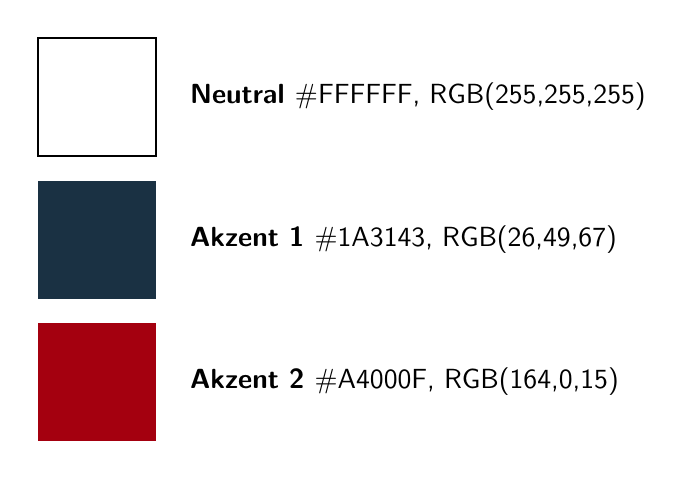
\begin{tikzpicture}
		\tikzstyle{colorswatch} = [rectangle,draw=none,minimum width=15mm,minimum height=15mm,thick];
		\tikzstyle{colorspec} = [draw=none,fill=none,right];

		\matrix[row sep=3mm, column sep=3mm]{
			\node[colorswatch,draw=black,fill=spec_white]{}; &
			\node[colorspec]{\sffamily\bfseries Neutral \normalfont\sffamily\#FFFFFF, RGB(255,255,255)}; \\
			\node[colorswatch,fill=spec_blue]{}; &
			\node[colorspec]{\sffamily\bfseries Akzent 1 \normalfont\sffamily\#1A3143, RGB(26,49,67)}; \\
			\node[colorswatch,fill=spec_red]{}; &
			\node[colorspec]{\sffamily\bfseries Akzent 2 \normalfont\sffamily\#A4000F, RGB(164,0,15)}; \\
		};
	\end{tikzpicture}
	\caption{Branding Farbpalette}
\end{figure}

\subsubsection*{Logo \& Logovariationen}
\begin{figure}[H]
	\centering
	
\includegraphics[width=5cm]{content/images/roomies-withshadow.png}
	\caption{Roomies Logo im College Stil}
\end{figure}

\begin{figure}[H]
	\centering
	
\includegraphics[width=10cm]{content/images/logo-variants.png}
	\caption{Roomies Logo in verschiedenen Grössen \& Varianten}
\end{figure}

\newpage
\section{Technologieevaluation}
Das Thema ``Architekturkonzepte moderner Web-Applikationen'' legt den Schluss nahe, nicht nur aktuellste Architekturprinzipien bei der Umsetzung der Beispielapplikation zu verwenden, sondern auch im Bereich der Technologiewahl auf etablierte Platzhirsche wie Java oder C\# (in Verbindung mit deren Web-Frameworks) zu verzichten.

Unter Berücksichtigung der persönlichen Erfahrungen und Einschätzungen aller Projektteilnehmer wurde in Vereinbarung mit dem Betreuer im Zuge einer Evaluation eine Shortlist mit folgenden Technologiekandidaten zusammengestellt:

\begin{itemize}
	\item \emph{Ruby}\\
	Ruby hat sich in der näheren Vergangenheit zusammen mit Ruby On Rails im Markt etablieren können. Als relativ junge Technologie durfte es aus diesem Grund bei einer Evaluation nicht ignoriert werden.

	\item \emph{Java}\\
	Trotz des einführenden Statements, Platzhirsche von einer engeren Auswahl auszuschliessen, war das Projektteam aufgrund der vorangegangenen Studienarbeit davon überzeugt, dass Java, insbesondere als Backendtechnologie, mit den ``jungen Wilden'' problemlos mithalten kann.

	\item \emph{JavaScript}\\
	Während den letzten zwei Jahren erlebte JavaScript eine Renaissance: Mit node.js schaffte es den Sprung vom Frontend-Layer ins Backend und erfreut sich in der OpenSource als auch der Industrie-Community grösster Beliebtheit.
\end{itemize}

In diesem Abschnitt werden übergreifende Bewertungskriterien definiert, welche anschliessend auf alle drei Technologiekandidaten, resp. deren Frameworks angwendet werden können.

\newpage
\subsection{Bewertungskriterien \& Gesamtbewertung}
Die folgende Tabelle definert sechs Kriterien, welche zur Bewertung einer Technologie oder eines Frameworks jeweils mit 0-3 Sternen bewertet werden können.

Die Spalte \emph{Gewichtung} gibt an, als wie wichtig das betreffende Kriterium im Bezug auf die Aufgabenstellung anzusehen ist.

\begin{table}[H]
\tablestyle
\tablealtcolored
\begin{tabularx}{\textwidth}{l l X c}
\tableheadcolor
	\tablehead ID &
	\tablehead Kriterium &
	\tablehead Erläuterung &
	\tablehead Gewichtung \tabularnewline
\tablebody
\textit{TK1} &
	Eigenkonzepte &
	Wieviele eigene Konzepte \& Ideen bringt eine Technologie resp. ein Framework mit? Viele spezifische Konzepte bedeuten meistens eine steile Lernkurve für Neueinsteiger. \emph{Hohe Bewertung = Wenig Eigenkonzepte}&
	\faStar\faStar\faStar \tabularnewline
\textit{TK2} &
	Eignung &
	Wie gut eignet sich eine Technologie oder ein Framework für die Demonstration der Architekturrichtlinien? Geschieht alles ``hinter'' dem Vorhang oder sind einzelne Komponenten einsehbar? \emph{Hohe Bewertung = Hohe Eignung}&
	\faStar\faStar\faStar \tabularnewline
\textit{TK3} &
	Produktreife &
	Wie gut hat sich das Framework oder die Technologie bis jetzt in der Realität beweisen können? Wie lange existiert es schon? Gibt es eine aktive Community und wird es aktiv weiterentwickelt? \emph{Hohe Bewertung = Hohe Produktreife}&
	\faStar\faStar\faStar\tabularnewline
\textit{TK4} &
	Aktualität &
	Diese Arbeit kümmert sich um ``moderne Web-Applikationen''. So sollte auch die zu verwendende Technologie gewissermassen nicht von ``vorgestern'' sein. \emph{Hohe Bewertung = Hohe Aktualität}&
	\faStar \tabularnewline
\textit{TK5} &
	``Ease of use'' &
	Wie angenehm ist das initiale Erstellen, die Konfiguration und die Unterhaltung einer Applikation? Führt das Framework irgendwelchen ``syntactic sugar'' \cite{syntacticsugar} ein um die Arbeit zu erleichtern? \emph{Hohe Bewertung = Hoher ``Ease of use''-Faktor} &
	\faStar\faStar \tabularnewline
\textit{TK6} &
	Testbarkeit &
	Wie gut können die mit dem Framework oder der Technologie erstellte Komponenten durch Unit Tests getestet werden? \emph{Hohe Bewertung = Hohe Testbarkeit} &
	\faStar\faStar \tabularnewline
\tableend
\end{tabularx}
\caption{Bewertungskriterien für Technologieevaluation}
\label{tab:bewertungskriterien}
\end{table}


Für jedes Framework wird abschliessend eine Gesamtbewertung in Form einer Zahl errechnet. Dies geschieht mit folgender Formel:

\begin{figure}[H]
	\centering
	\large
	\begin{math}
		\frac{\sum \limits_{n=1}^6 Bewertung_{TK_n} \times {Gewichtung_{TK_n}}}{6}
	\end{math}
	\caption{Berechnungsformel Gesamtbewertung}
\end{figure}


\newpage
\subsection{Ruby}

Insbesondere mit dem Framework \emph{Ruby on Rails} \cite{RubyOnRails} wurde Ruby für die Entwicklung von Umfangreichen Webapplikationen seit Veröffentlichung in den 90ern immer beliebter. Mit fast kindlicher Selbstverständlichkeit bringt Ruby viele Konzepte wie \gls{Multiple Inheritance} (in Form von Mixins) oder die funktionale Behandlung von jeglichen Werten/Objekten von Haus aus mit.

Für den Einsteiger etwas verwirrend setzt es zudem auf eine für den Menschen ``leserlichere'' Syntax als beispielsweise von Java oder anderen verwandten Sprachen gewohnt. Folgende Codebeispiele bewirken die selbe Ausgabe auf der Kommandozeile, unterscheiden sich aber deutlich in ihrer Formulierung:

\begin{lstlisting}[language=Java, caption=Negierte if-Abfrage in Java]
if(!enabled) {
	System.out.println("Ich bin deaktiviert!");
}
\end{lstlisting}

\begin{lstlisting}[language=Ruby, caption=Negierte if-Abfrage in Ruby]
puts "Ich bin deaktiviert!" unless enabled
\end{lstlisting}

Während der kurzen Technologieevaluationsphase wurde im Bereich Ruby das Hauptaugenmerk auf \emph{Ruby on Rails} gelegt. Insbesondere die \gls{Scaffolding}tools und der daraus generierte Quellcode wurde näher begutachtet. Die Resultate sind wiederum auf die sechs Bewertungskriterien appliziert worden.

\subsubsection*{Bewertung Ruby on Rails}
\begin{table}[H]
\newcolumntype{s}{>{\centering\hsize=0.15\hsize}X}
\tablestyle
\tablealtcolored
\begin{tabularx}{\textwidth}{X s s s s s s s}
\tableheadcolor
	\tablehead &
	\rotatebox{90}{\bfseries\textit{TK1 Eigenkonzepte} } &
	\rotatebox{90}{\bfseries\textit{TK2 Eignung}} &
	\rotatebox{90}{\bfseries\textit{TK3 Produktreife}} &
	\rotatebox{90}{\bfseries\textit{TK4 Aktualität}} &
	\rotatebox{90}{\bfseries\textit{TK5 ``Ease of use''}} &
	\rotatebox{90}{\bfseries\textit{TK6 Testbarkeit}} &
	\rotatebox{90}{\bfseries\textit{Gesamtbewertung}}
	\tabularnewline
\tablebody
	\textit{Ruby on Rails} &
	\oneStar &
	\oneStar &
	\threeStars &
	\oneStar &
	\threeStars &
	\twoStars &
	\directlua{
		tex.print(math.round(
			(1 * 3 +
			1 * 3 +
			3 * 3 +
			1 * 1 +
			3 * 2 +
			2 * 2) / 6
		))
	}
	\tabularnewline
\tableend
\end{tabularx}
\caption{Bewertung Ruby on Rails}
\end{table}


\subsubsection*{Interpretation}
Nach genauerem Befassen mit Ruby on Rails sind die Einschätzung des Projektteams gespalten.

Zum Einen minimiert Ruby on Rails den Aufwand für das Erledigen von Routineaufgaben extrem (\gls{Scaffolding}). Der generierte Code ist sofort verwendbar und, gute Ruby-Kenntnisse vorausgesetzt, gut erweiterbar.

Zum Anderen ist aber gerade die Einfachheit, wie bspw. Controllers oder Models erzeugt und in den Applikationsablauf eingebunden werden, alles Andere als optimal wenn es darum geht, Architekturrichtlinien eindeutig und klar demonstrieren zu können.

Unter dem Vorbehalt, dass Ruby on Rails für die Demonstration der definierten Architekturrichtlinien evtl. nicht die richtige Wahl sein könnte, kann das Projektteam nur eine bedingte Empfehlung für das Ruby Framework abgeben.

\subsection{Java}

Schon vor dieser Bachelorarbeit kann das Projektteam diverse Erfahrungen mit Java vorweisen. Zum Einen aus privaten und beruflichen Projekten, zum Anderen auch ganz themenspezifisch aus der Studienarbeit, welche ein Semester früher durchgeführt wurde.

Als Teil einer grösseren Applikation wurde dort ein Webservice mit REST-Schnittstelle umgesetzt. Zum Einsatz kamen diverse Referenzimplementierungen von Java Standard API's. Die sehr positiven Erfahrungen mit der dort orchestrierten Zusammenstellung von Bibliotheken legen den Schluss nahe, diese auch für eine potentielle Verwendung innerhalb dieser Bachelorarbeit wiederzuverwenden.

Der Studienarbeit-erprobten Kombination sollen jedoch auch andere Alternativen gegenübergestellt werden. Insgesamt ergeben sich so folgende Analysekandidaten im Bereich der Technologie \emph{Java}:

\begin{table}[H]
\tablestyle
\tablealtcolored
\begin{tabularx}{\textwidth}{l X l}
\tableheadcolor
	\tablehead Framework &
	\tablehead Erläuterung \tabularnewline
\tablebody
\textit{Studienarbeit-Zusammenstellung} &
	Die Zusammenstellung von \emph{Google Guice}, \emph{Jersey}, \emph{Codehaus Jackson} sowie \emph{EclipseLink} hat sehr gut harmoniert. Die Verwendung von einem Java-fremden Framework für die Implementierung des Frontends wäre jedoch erneut abzuklären.
	\tabularnewline
\textit{Spring} &
	Spring hat sich in den letzten Jahren in der Industrie etablieren können. Es bietet eine Vielzahl von Subkomponenten (MVC, Beanmapping etc.).
	\tabularnewline
\textit{Plain JEE} &
	Java Enterprise bietet von sich aus viele Features, welche die Frameworks von Dritten unter anderen Ansätzen umsetzen. Es gilt jedoch abzuwägen, wie gross der Aufwand ist, um beispielsweise eine REST-Serviceschnittstelle zu implementieren.
	\tabularnewline
\textit{Vaadin} &
	Vaadin baut auf Googles GWT und erlaubt die serverlastige Entwicklung von Webapplikationen.
	\tabularnewline
\textit{Play! Framework} &
	Seit dem Release der Version 2.0 im Frühjar 2012 erfreut sich das Play! Frameworks grosser Beliebtheit. Insbesondere die integrierten Scaffolding-Funktionalitäten und MVC-Ansätze werden gelobt.
	\tabularnewline
\tableend
\end{tabularx}
\caption{Shortlist Analysekandidaten Java}
\end{table}


\subsubsection*{Bewertungsmatrix}

\begin{table}[H]
\newcolumntype{s}{>{\centering\hsize=0.15\hsize}X}
\tablestyle
\tablealtcolored
\begin{tabularx}{\textwidth}{X s s s s s s s}

\tableheadcolor
	\tablehead &
	\rotatebox{90}{\bfseries\textit{TK1 Eigenkonzepte} } &
	\rotatebox{90}{\bfseries\textit{TK2 Eignung}} &
	\rotatebox{90}{\bfseries\textit{TK3 Produktreife}} &
	\rotatebox{90}{\bfseries\textit{TK4 Aktualität}} &
	\rotatebox{90}{\bfseries\textit{TK5 ``Ease of use''}} &
	\rotatebox{90}{\bfseries\textit{TK6 Testbarkeit}} &
	\rotatebox{90}{\bfseries\textit{Total}}
	\tabularnewline
\tablebody
	\textit{Studienarbeit-Zusammenstellung}	&
	\threeStars &
	\threeStars &
		&
		&
	\threeStars &
	\twoStars &
	\directlua{
		tex.print(math.round(
			(3 * 3 +
			3 * 3 +
			0 * 3 +
			0 * 1 +
			3 * 2 +
			2 * 1) / 6
		))
	}
	\tabularnewline


	\textit{Spring} &
		&
		&
	\twoStars &
	\threeStars &
		&
	\oneStar &
	\directlua{
		tex.print(math.round(
			(0 * 3 +
			0 * 3 +
			2 * 3 +
			3 * 1 +
			0 * 2 +
			1 * 1) / 6
		))
	}
	\tabularnewline


	\textit{Plain JEE} &
		&
	\twoStars &
	\threeStars &
	\threeStars &
		&
	\threeStars &
	\directlua{
		tex.print(math.round(
			(0 * 3 +
			2 * 3 +
			3 * 3 +
			3 * 1 +
			0 * 2 +
			3 * 1) / 6
		))
	}
	\tabularnewline


	\textit{Vaadin} &
	\oneStar &
		&
	\threeStars &
	\twoStars &
		&
	\threeStars &
	\directlua{
		tex.print(math.round(
			(1 * 3 +
			0 * 3 +
			3 * 3 +
			2 * 1 +
			0 * 2 +
			3 * 1) / 6
		))
	}
	\tabularnewline


	\textit{Play! Framework} &
	\oneStar &
	&
	\twoStars &
	\twoStars &
	&
	\threeStars&
	\directlua{
		tex.print(math.round(
			(1 * 3 +
			0 * 3 +
			2 * 3 +
			2 * 1 +
			0 * 2 +
			3 * 1) / 6
		))
	}
	\tabularnewline
\tableend
\end{tabularx}
\caption{Bewertungsmatrix Java Frameworks}
\end{table}

\subsubsection*{Interpretation}
\emph{Plain JEE}, \emph{Vaadin} und \emph{Play! Framework} spielen ihre Stärken klar in der Produktreife und der dadurch hohen Wartbarkeit resp. Testbarkeit aus. Im Bezug auf die Eigenkonzepte benötigen alle Kandidaten einen gewissen initialen Lernaufwand. \emph{Studienarbeit-Zusammenstellung} arbeitet mit einem klar zugänglichen Schichtenmodell und verwendet über dies hinaus ein komplett vom Backend entkoppeltes Frontend. Zwar wäre eine solche Lösung auch mit \emph{Spring} und \emph{Plain JEE} möglich, jedoch versagen diese beiden Frameworks wiederum im Bezug auf die Eignung, die aufgestellten Architekturrichtlinien transparent demonstrieren zu können.

Die Produktreife von \emph{Studienarbeit-Zusammenstellung} ist zu vernachlässigen. Die einzelnen Komponenten für sich haben sich bereits in länger in der Praxis bewähren können und sind lediglich genau in dieser Kombination evtl. weniger oft erprobt.

Für die endgültige Auswahl einer Technologie schickt Java aufgrund vorangegangener Bewertung die \emph{Studienarbeit-Zusammenstellung} in die finale Ausscheidung.

\subsection{JavaScript}
\label{sec:technology-evaluation-javascript}

JavaScript ist insbesondere als ``Webprogrammiersprache'' bekannt. In den vergangenen Jahren wurde es hauptsächlich innerhalb des Internetbrowsers verwendet, um starre Internetseiten mit mehr Interaktivität zu versehen. Insbesondere die Anstrengungen von Mozilla \cite{SpiderMonkey} und Google \cite{V8JavaScript} verhalfen der früher für schlechte Performance und schlechte Codequalität verschrieenen Programmiersprache zu neuem Glanz.

Mit JavaScript sind heute innerhalb des Browsers komplexe und umfangreiche Applikationen problemlos umzusetzen und weit verbreitet.

Die quelloffene V8 JavaScript Engine \cite{V8JavaScript} von Google hat 2009 zudem den Sprung weg vom Browser geschafft: node.js \cite{nodejs} bietet die Engine als eigenständigen Skriptinterpreter an und verfügt über eine umfangreiche, leistungsstarke und systemnahe API. Die neu entstandene Plattform erfreut sich in der Opensource Community grösster Beliebtheit. So sind seit der ersten Veröffentlichung eine Vielzahl an Frameworks und Bibliotheken zu den verschiedensten Themengebieten entstanden.

Auch im Bereich der Webframeworks gibt es auf diese Weise eine Menge an interessanten Libraries zu entdecken. Für die Evaluation im Bezug auf diese Bachelorarbeit werden folgende Frameworks genauer analysiert:

\begin{table}[H]
\tablestyle
\tablealtcolored
\begin{tabularx}{\textwidth}{l X l}
\tableheadcolor
	\tablehead Framework &
	\tablehead Erläuterung \tabularnewline
\tablebody
\textit{Express.js} &
	Express.js \cite{Expressjs} baut auf dem Basisframework Connect \cite{connect} auf. Das damit durchgängig umgesetzte Middleware-Konzept ermöglicht die entkoppelte Entwicklung von simplen Webservern bis hin ausgefeilten Webservices. Zu Beginn genügen max. 10 Zeilen Quellcode, um einen GET-Request \cite{HTTPRequest} entgegen zu nehmen und eine Antwort an den Aufrufer zurück zu senden. Dem Ausbau zu komplexeren Applikationen steht dank der erwähnten Middleware-Architektur jedoch nichts im Wege.
	\tabularnewline
\textit{Tower.js} &
	Pate für Tower.js \cite{towerjs} steht nach eigenen Angaben des Entwicklers Ruby on Rails. Entsprechend umfangreich sind auch hier die \gls{Scaffolding}funktionalitäten. Das Framework selbst ist mit CoffeeScript \cite{CoffeeScript} entwickelt worden. Wie das Ruby-Vorbild bietet auch Tower.js ein ausgewachsenes MVC-Pattern zur Entwicklung eigener Applikationen an.
	\tabularnewline
\textit{derby} &
	Das Framework Derby \cite{Derby} nimmt sich das oben eingeführte Express.js zur Grundlage und erweitert es im das Model-View-Controller-Pattern. Es bleibt dabei extrem leichtgewichtig, ermöglicht aber leider keine Browserclients welche der Anforderung des \emph{Unobtrusive JavaScripts} genügen mögen: Derby-Applikationen werden komplett im Browser gerendert und bieten keine Möglichkeit, HTML-Markup auf dem Server zu generieren.
	\tabularnewline
\textit{Geddy} &
	Mit Geddy \cite{Geddy} begibt sich bereits der zweite Kandidat für node.js in den Ring, welcher sich Ruby on Rails zum Vorbild nimmt. Dementsprechend vergleichbar ist der Funktionsumfang mit Tower.js. Als wichtiger Unterschied ist jedoch zu erwähnen, dass Geddy auf CoffeeScript vollends verzichtet.
	\tabularnewline
\textit{Sails} &
	Sails \cite{sails} ist der jüngste Frameworkkandidat für JavaScript resp. node.js. Die Grundkonzepte von Ruby on Rails werden mit einer Prise ``Realtime'' (\glspl{Websocket}) gewürzt. So kann jede Ressource über eine einfache REST-Schnittstelle als auch über eine Websocket-Verbindung angesprochen werden. Damit erleichtert sich das asynchrone resp. servergesteuerte Aktualisieren des Frontends.
	\tabularnewline
\tableend
\end{tabularx}
\caption{Shortlist Analysekandidaten JavaScript}
\end{table}



\subsubsection*{Bewertungsmatrix}

\begin{table}[H]
\newcolumntype{s}{>{\centering\hsize=0.15\hsize}X}
\tablestyle
\tablealtcolored
\begin{tabularx}{\textwidth}{X s s s s s s s}
\tableheadcolor
	\tablehead &
	\rotatebox{90}{\bfseries\textit{TK1 Eigenkonzepte} } &
	\rotatebox{90}{\bfseries\textit{TK2 Eignung}} &
	\rotatebox{90}{\bfseries\textit{TK3 Produktreife}} &
	\rotatebox{90}{\bfseries\textit{TK4 Aktualität}} &
	\rotatebox{90}{\bfseries\textit{TK5 ``Ease of use''}} &
	\rotatebox{90}{\bfseries\textit{TK6 Testbarkeit}} &
	\rotatebox{90}{\bfseries\textit{Total}}
	\tabularnewline
\tablebody
	\textit{Express.js}	&
	\threeStars &
	\threeStars	&
	\twoStars &
	\threeStars &
	\twoStars &
	\threeStars &
	\directlua{
		tex.print(math.round(
			(3 * 3 +
			3 * 3 +
			2 * 3 +
			3 * 1 +
			2 * 2 +
			3 * 2) / 6
		))
	}
	\tabularnewline

	\textit{Tower.js} &
	\twoStars &
	\twoStars &
	\oneStar &
	\threeStars &
	\threeStars	&
		&
	\directlua{
		tex.print(math.round(
			(2 * 3 +
			2 * 3 +
			1 * 3 +
			3 * 1 +
			3 * 2 +
			0 * 2) / 6
		))
	}
	\tabularnewline


	\textit{derby} &
	\twoStars &
	\oneStar &
	\oneStar &
	\threeStars &
	\twoStars &
		&
	\directlua{
		tex.print(math.round(
			(2 * 3 +
			1 * 3 +
			1 * 3 +
			3 * 1 +
			2 * 2 +
			0 * 2) / 6
		))
	}
	\tabularnewline


	\textit{Geddy} &
	\threeStars &
	\oneStar &
	\twoStars &
	\twoStars &
	\threeStars &
	&
	\directlua{
		tex.print(math.round(
			(3 * 3 +
			1 * 3 +
			2 * 3 +
			2 * 1 +
			3 * 2 +
			0 * 2) / 6
		))
	}
	\tabularnewline


	\textit{Sails} &
	\twoStars &
	\twoStars &
	\oneStar &
	\threeStars &
	\twoStars &
	\oneStar &
	\directlua{
		tex.print(math.round(
			(2 * 3 +
			2 * 3 +
			1 * 3 +
			3 * 1 +
			2 * 2 +
			1 * 2) / 6
		))
	}
	\tabularnewline
\tableend
\end{tabularx}
\caption{Bewertungsmatrix JavaScript Frameworks}
\end{table}



\newpage
\section{Proof of Concept}
\label{sec:proof-of-concept}

In der Technologieevaluation zu \nameref{sec:technology-evaluation-javascript} stachen die beiden Frameworks Express.js \cite{Expressjs}
und Sails.js \cite{sails} heraus.

Obwohl Express.js stabiler ist und weitaus mehr genutzt wird, ist Sails.js aufgrund der neuen Ideen und interessanten Ansätzen für einen ersten Prototyp ausgewählt worden.

\subsection{Prototyp mit Sails.js}
Um sich ein Bild von Sails.js zu machen wurde ein einfacher Prototyp \cite{SailsPrototyp} erstellt.

Sails.js verwendet \gls{Scaffolding} um einerseits ein neues Projekt zu erstellen, andererseits auch um verschiedene Komponenten wie Model oder Controller zu erstellen. Wie im \nameref{sec:erdiagramm} beschrieben, werden u.a. ein Task und ein Resident Model (sowie entsprechende Tabelle) benötigt.

Um das \gls{ORM} ``Waterline'' \cite{Waterline} zu testen, wurden diese beiden Models implementiert. Das Task-Model mittels Sails.js definiert sieht so aus:

\begin{lstlisting}[language=JavaScript, caption=Task Model in Sails.js (Name wird durch Dateiname definiert.)]
module.exports = {
	attributes: {
		name: "string"
		, description: "string"
		, points: "int"
		, userId: "int"
		, communityId: "int"
	}
};
\end{lstlisting}

Mit einer Definition eines Models wird automatisch eine \gls{REST}-API für dieses erstellt.

Damit lassen sich einerseits CRUD-Operationen direkt über HTTP ausführen, andererseits existiert auch die Möglichkeit Socket.IO \cite{SocketIO} zu aktivieren, um Models direkt von einem offenen \gls{Websocket} zu verwenden.

Dieses Feature macht Sails.js sehr nützlich für \gls{Realtime}-Applikationen.

Um eine effektive HTML-Seite darstellen zu können wird ein Controller sowie eine View benötigt. Dies wurde im Prototyp für Aufgaben (Tasks) implementiert.

\begin{lstlisting}[language=JavaScript, caption=Task Controller in Sails.js, label=lst:sailsjstaskcontroller]
var TaskController = {
	get: function(req, res) {
		var id = req.param('id');
		Task.find(id).done(function(err, task) {
			User.find(task.userId).done(function(err, user) {
				var response = {
					'task': task,
					'user': user,
					'title': task.name
				};

				if (req.acceptJson) {
					res.json(response);
				} else if(req.isAjax && req.param('partial')) {
					response['layout'] = false;
					res.view(response);
				} else {
					res.view(response);
				}
			});
		});
	}

};
module.exports = TaskController;
\end{lstlisting}

In diesem Controller wird ein Task aufgrund des GET-Parameters ``id'' (Linien 3 und 4) geladen. Das Code-Stück zeigt die grosse Schwäche des ORMs Waterline \cite{Waterline}. Statt dass man auf dem ``task''-Objekt direkt ``.user'' aufrufen könnte, muss man den Umweg über ``User.find()'' gehen.

Bei einem ausgereiften ORM würden solche Methoden wegen der Definition von Relationen direkt zur Verfügung stehen.

Der Controller antwortet auf eine Anfrage eines Browsers mit folgendem HTML:

\begin{lstlisting}[language=HTML, caption=Task Template]
<div id="task-display">
	<h1>Task: <%= task.name %></h1>
	<ul>
		<li>Points: <%= task.points %></li>
		<li>Created At: <%= task.createdAt %></li>
	</ul>
	<h2>User: <%= user.name %></h2>
	<ul>
		<li>Created At: <%= user.createdAt %></li>
	</ul>
</div>
<a href="#" id="reload">Reload!</a>
<script>
	$('#reload').on('click', function() {
		$.ajax('/task/get/?id=<%= task.id %>&partial=true', {
			success: function(response) {
				var $response = $('<div class="body-mock">' + response + '</div>');
				html = $response.find('#task-display');
				$('#task-display').replaceWith(html);
			}
		});
	});
</script>
\end{lstlisting}

Mit dem einfachen Script am Schluss des Task Templates wird aufgezeigt, wie man ohne Neuladen der Seite direkt HTML ersetzen kann. Dies ist grundsätzlich Framework-unabhängig und es wurde dabei auch nicht auf ``RP14'' (Unobtrusive JavaScript) Wert gelegt.

\subsubsection*{Schlussfolgerung}

Wie bereits vorher angemerkt, ist das ORM von Sails.js nicht ausgereift. Weder Assoziationen zwischen Models \cite{SailsjsModelAssociations} noch das setzen von Indizes ist möglich.

Für das Resident-Model ist es u.a. auch nötig, Facebook IDs zu speichern. Diese sind 64 Bit gross und wegen mangelhafter Unterstützung des ORMs wäre das gar nicht möglich.

Nebst dem ORM ist auch das Framework und die zugehörige Dokumentation wenig umfangreich. Auch die Community war zum Zeitpunkt der Evaluation (siehe Anhang \ref{sec:appendix-technology-evaluation} zur \nameref{sec:appendix-technology-evaluation}) sehr klein. Die Fakten deuten sehr darauf hin, Sails.js nicht für die konkrete Beispielapplokation zu verwenden. Aus diesem Grund soll ein zweiter Prototyp unter Verwendung von Express.js erstellt werden.
\subsection{Prototyp mit Express.js}

Express.js \cite{Expressjs} ist ein leichtgewichtiges Framework, welches mittels Connect-Middlewares \cite{connect} erweitert werden kann.

Damit die Eignung von Express.js überprüft werden kann, wurde ebenfalls ein Prototyp \cite{ExpressjsPrototyp} erstellt.

Der initiale Startpunkt des Express.js Prototyps ist die Datei ``app.js'' \cite{ExpressjsPrototypAppjs}. Dort werden alle benutzten Middlewares registriert, die Datenbank aufgesetzt und Controller registriert.

Ein Beispielhafter Controller ist im Quelltext \ref{lst:controllerInExpressjs} zu sehen.

\begin{lstlisting}[language=JavaScript, caption=Beispiel eines Controllers in Express.js, label=lst:controllerInExpressjs]
exports.index = function(req, res){
	// first Parameter: Template File to use
	// 2nd Parameter: Context to pass to the template
	res.render('index', { title: 'Express' });
};
\end{lstlisting}

Ein zugehöriges Template kann folgendermassen aussehen:

\begin{lstlisting}[language=HTML, caption=Template in Express.js, label=lst:templateInExpressjs]
<!DOCTYPE html>
<html>
	<head>
		<title><%= title %></title>
		<link rel='stylesheet' href='/stylesheets/style.css' />
		<%- LRScript %>
	</head>
	<body>
		<h1><%= title %></h1>
		<p>Welcome to <%= title %></p>
	</body>
</html>
\end{lstlisting}

In den vorangegangenen zwei Quellcode-Listings \ref{lst:controllerInExpressjs} und \ref{lst:templateInExpressjs} ist ersichtlich, dass der Applikationsentwickler sehr grosse Kontrolle über Express.js hat.

Die Flexiblilität von Express.js bietet sowohl Vor- als auch Nachteile für die erstellung von Webapplikationen. Im Bezug auf die Veranschaulichung der \nameref{sec:architekturrichtlinien} ist es jedoch ein grosser Vorteil, da wenig Logik fix in Express.js eingebaut ist.
\subsubsection{\gls{ORM}}
Im Gegensatz zu den anderen evaluierten Frameworks ist bei Express.js kein ORM enthalten. Deswegen musste auch bzgl. des ORMs eine kurze Evaluation gemacht werden.
Tabelle \ref{tab:bewertungskriterienORM} zeigt die Kriterien und Gewichtung für die Evaluation des ORMs.

\begin{table}[H]
\tablestyle
\tablealtcolored
\begin{tabularx}{\textwidth}{l l X c}
\tableheadcolor
	\tablehead ID &
	\tablehead Kriterium &
	\tablehead Erläuterung &
	\tablehead Gewichtung \tabularnewline
\tablebody
\textit{OK1} &
	Unterstützung DBs &
	Wieviele unterschiedliche Datenbanken unterstützt das ORM? Werden auch \gls{NoSQL}-Datenbanken unterstützt? \emph{Hohe Bewertung = Grosse Anzahl an Datenbanken}&
	\faStar \tabularnewline
\textit{OK2} &
	Relationen &
	Sind Relationen definierbar zwischen Tabellen? Verwenden diese die Datenbank-spezifischen Foreign Keys dafür (falls möglich)? \emph{Hohe Bewertung = Relationen möglich und verwendet Datenbank-spezifische Datentypen}&
	\faStar\faStar\faStar \tabularnewline
\textit{OK3} &
	Produktreife &
	Wie gut hat sich das ORM bis jetzt in der Realität beweisen können? Wie lange existiert es schon? Gibt es eine aktive Community und wird es aktiv weiterentwickelt? \emph{Hohe Bewertung = Hohe Produktreife}&
	\faStar\faStar\faStar\tabularnewline
\textit{OK4} &
	``Ease of use'' &
	Wie angenehm ist das initiale Erstellen, die Konfiguration und die Unterhaltung von Models? Führt das ORM irgendwelchen ``syntactic sugar'' \cite{syntacticsugar} ein um die Arbeit zu erleichtern? \emph{Hohe Bewertung = Hoher ``Ease of use''-Faktor} &
	\faStar \tabularnewline
\textit{OK5} &
	Testbarkeit &
	Wie gut können die mit dem Framework oder der Technologie erstellte Komponenten durch Unit Tests getestet werden? \emph{Hohe Bewertung = Hohe Testbarkeit} &
	\faStar\faStar \tabularnewline
\tableend
\end{tabularx}
\caption{Bewertungskriterien für ORM-Evaluation}
\label{tab:bewertungskriterienORM}
\end{table}


\begin{table}[H]
\newcolumntype{s}{>{\centering\hsize=0.15\hsize}X}
\tablestyle
\tablealtcolored
\begin{tabularx}{\textwidth}{X s s s s s s}
\tableheadcolor
	\tablehead &
	\rotatebox{90}{\bfseries\textit{OK1 Unterstützung DBs} } &
	\rotatebox{90}{\bfseries\textit{OK2 Relationen}} &
	\rotatebox{90}{\bfseries\textit{OK3 Produktreife}} &
	\rotatebox{90}{\bfseries\textit{OK4 ``Ease of use''}} &
	\rotatebox{90}{\bfseries\textit{OK5 Testbarkeit}} &
	\rotatebox{90}{\bfseries\textit{Total}}
	\tabularnewline
\tablebody
	\textit{JugglingDB} &
	\threeStars &
	\oneStar &
	\oneStar &
	\twoStars &
	\twoStars &
	\directlua{
		tex.print(math.round(
			(3 * 1 +
			1 * 3 +
			1 * 3 +
			2 * 1 +
			2 * 2) / 5
		))
	}
	\tabularnewline

	\textit{Node-ORM2} &
	\twoStars &
	\twoStars	&
	\oneStar &
	\threeStars &
	\oneStar &
	\directlua{
		tex.print(math.round(
			(2 * 1 +
			2 * 3 +
			1 * 3 +
			3 * 1 +
			1 * 2) / 5
		))
	}
	\tabularnewline

	\textit{Sequelize} &
	\oneStar &
	\twoStars &
	\twoStars &
	\twoStars &
	\oneStar &
	\directlua{
		tex.print(math.round(
			(1 * 1 +
			2 * 3 +
			2 * 3 +
			2 * 1 +
			1 * 2) / 5
		))
	}
	\tabularnewline
\tableend
\end{tabularx}
\caption{Bewertungsmatrix JavaScript ORMs}
\label{tab:bewertungsmatrixORM}
\end{table}

Alle verglichenen ORMs haben eine ähnliche Gesamtbewertung. Bei ``Sequelize'' stechen jedoch die Produktreife und die Unterstützung für Relationen heraus.

Diese zwei Gründe zusammen mit der Roadmap \cite{RoadmapSequelize} von Sequelize haben schliesslich zur Überzeugung geführt, dass Sequelize die richtige Wahl ist.
